\documentclass[letterpaper,12pt]{article}
\usepackage{array}
\usepackage{threeparttable}
\usepackage{geometry}
\geometry{letterpaper,tmargin=1in,bmargin=1in,lmargin=1.25in,rmargin=1.25in}
\usepackage{fancyhdr,lastpage}
\pagestyle{fancy}
\lhead{}
\chead{}
\rhead{}
\lfoot{}
\cfoot{}
\rfoot{\footnotesize\textsl{Page \thepage\ of \pageref{LastPage}}}
\renewcommand\headrulewidth{0pt}
\renewcommand\footrulewidth{0pt}
\usepackage[format=hang,font=normalsize,labelfont=bf]{caption}
\usepackage{listings}
\lstset{frame=single,
  language=Python,
  showstringspaces=false,
  columns=flexible,
  basicstyle={\small\ttfamily},
  numbers=none,
  breaklines=true,
  breakatwhitespace=true
  tabsize=3
}
\usepackage{amsmath}
\usepackage{amssymb}
\usepackage{amsthm}
\usepackage{harvard}
\usepackage{setspace}
\usepackage{float,color}
\usepackage{graphicx}
\usepackage{hyperref}
\hypersetup{colorlinks,linkcolor=red,urlcolor=blue}
\theoremstyle{definition}
\newtheorem{theorem}{Theorem}
\newtheorem{acknowledgement}[theorem]{Acknowledgement}
\newtheorem{algorithm}[theorem]{Algorithm}
\newtheorem{axiom}[theorem]{Axiom}
\newtheorem{case}[theorem]{Case}
\newtheorem{claim}[theorem]{Claim}
\newtheorem{conclusion}[theorem]{Conclusion}
\newtheorem{condition}[theorem]{Condition}
\newtheorem{conjecture}[theorem]{Conjecture}
\newtheorem{corollary}[theorem]{Corollary}
\newtheorem{criterion}[theorem]{Criterion}
\newtheorem{definition}[theorem]{Definition}
\newtheorem{derivation}{Derivation} % Number derivations on their own
\newtheorem{example}[theorem]{Example}
\newtheorem{exercise}[theorem]{Exercise}
\newtheorem{lemma}[theorem]{Lemma}
\newtheorem{notation}[theorem]{Notation}
\newtheorem{problem}[theorem]{Problem}
\newtheorem{proposition}{Proposition} % Number propositions on their own
\newtheorem{remark}[theorem]{Remark}
\newtheorem{solution}[theorem]{Solution}
\newtheorem{summary}[theorem]{Summary}
%\numberwithin{equation}{section}
\bibliographystyle{aer}



\begin{document}

\begin{flushleft}
  \textbf{\large{Problem Set 4}} \\
  MACS 40000, Dr. Evans \\
  Sophia Mo
\end{flushleft}

\vspace{5mm}

\noindent\textbf{Problem 1(a)}\\
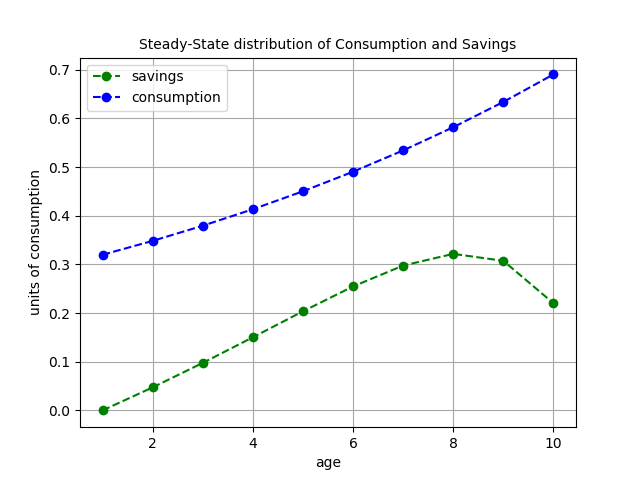
\includegraphics[scale=0.5]{ss_bc.png}
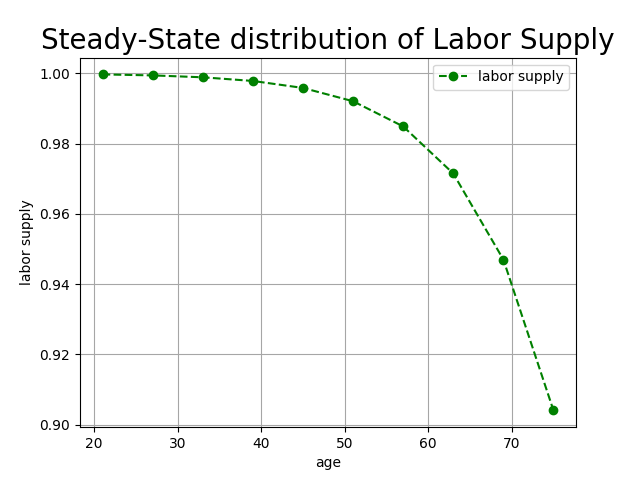
\includegraphics[scale=0.5]{ss_n}\\
\\
\noindent\textbf{Problem 1(b)}\\
\begin{table}[htbp!]\centering
\begin{tabular}{|l|c|}\hline
 $\bar{r}$ & 0.67\\
 $\bar{w}$ & 0.37\\
 $\bar{K}$ & 1.90\\
 $\bar{L}$ &9.70\\
 $\bar{Y}$ &5.48\\
 $\bar{C}$ &4.84\\
 Savings Euler Error & $3.55e^{-15}$\\
 Labor Euler Error & $3.19e^{-13}$\\
 Last period saving & $-1.29e^{-13}$\\
 Resource Constraint Error & $-2.01e^{-13}$\\ \hline
\end{tabular}
\end{table}
\\
\noindent\textbf{Problem 2(a)}\\
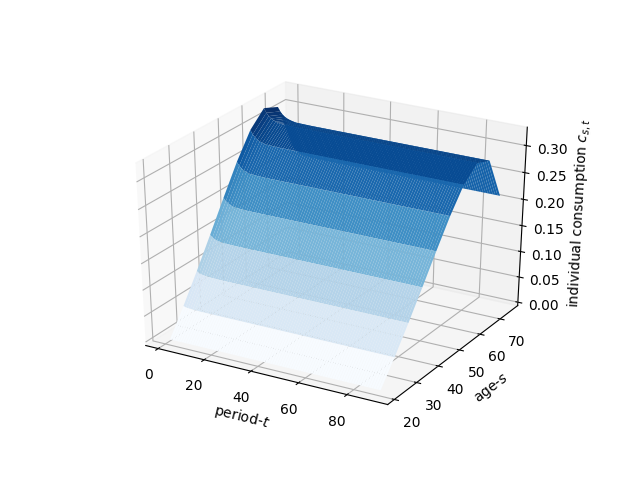
\includegraphics[scale=0.35]{cpath}
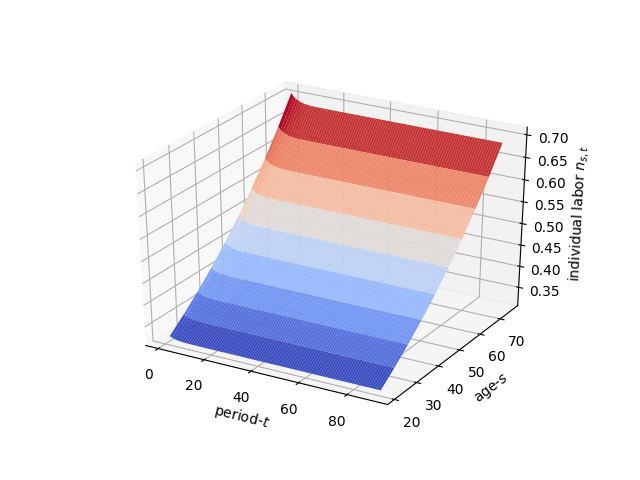
\includegraphics[scale=0.35]{npath}
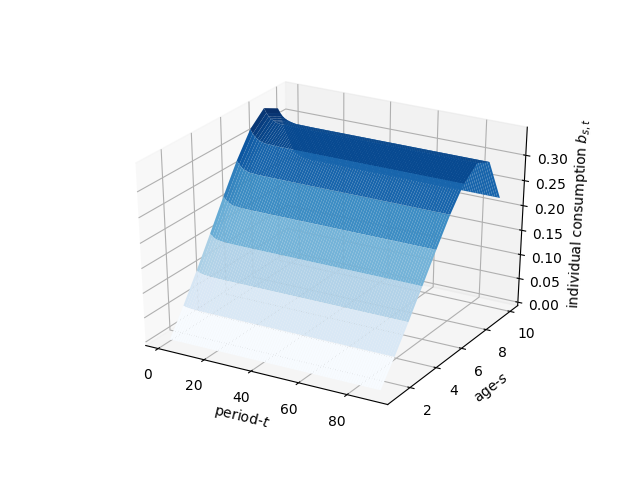
\includegraphics[scale=0.35]{bpath}
\\
\noindent\textbf{Problem 2(b)}\\
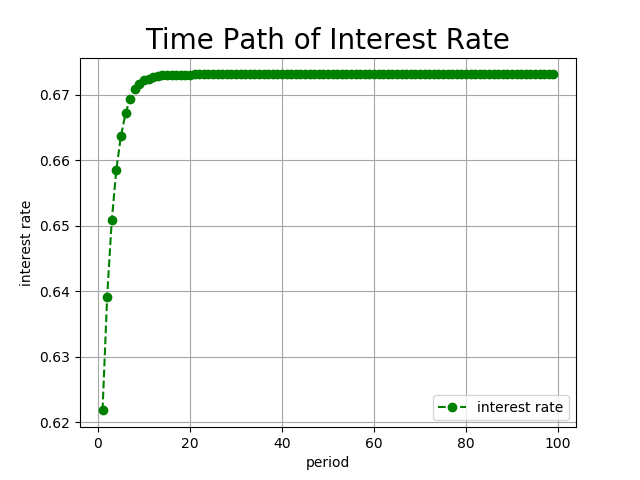
\includegraphics[scale=0.35]{tpi_r}
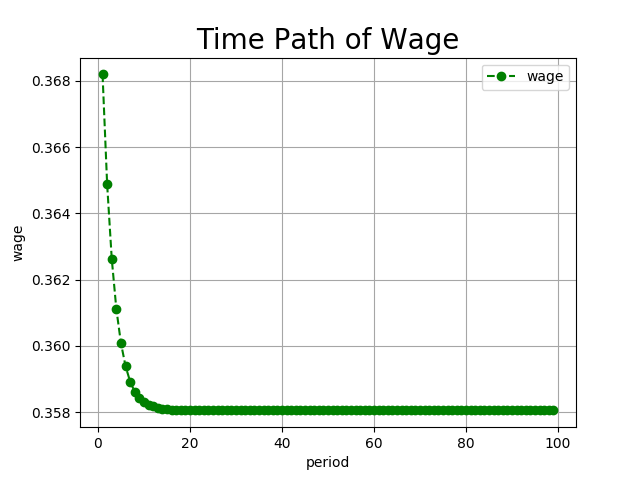
\includegraphics[scale=0.35]{tpi_w}
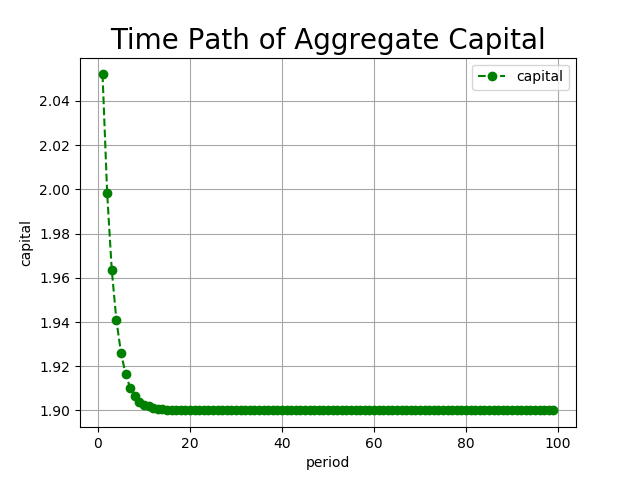
\includegraphics[scale=0.35]{tpi_K}
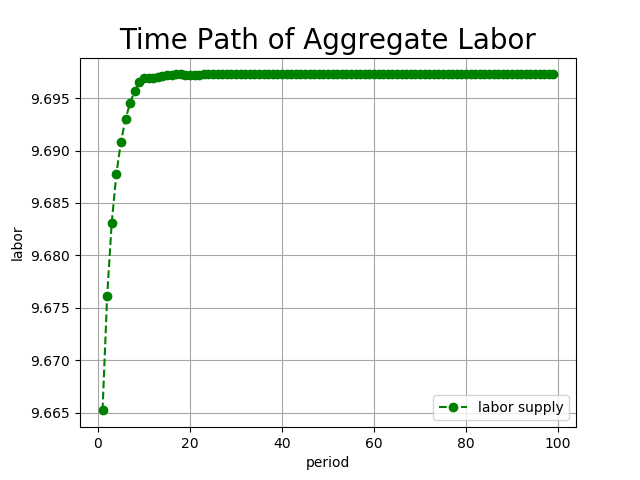
\includegraphics[scale=0.35]{tpi_L}
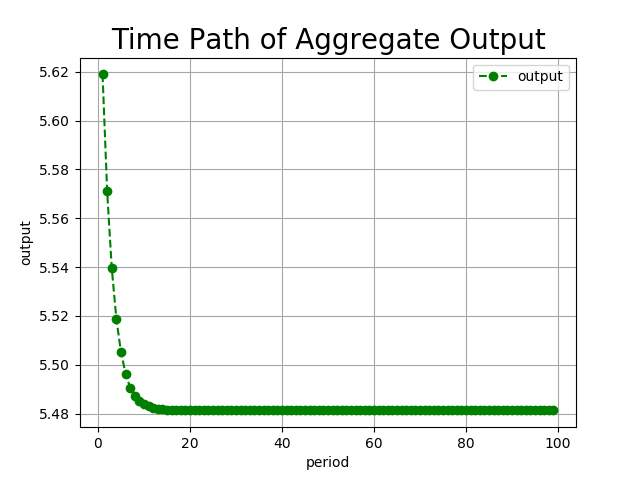
\includegraphics[scale=0.35]{tpi_Y}
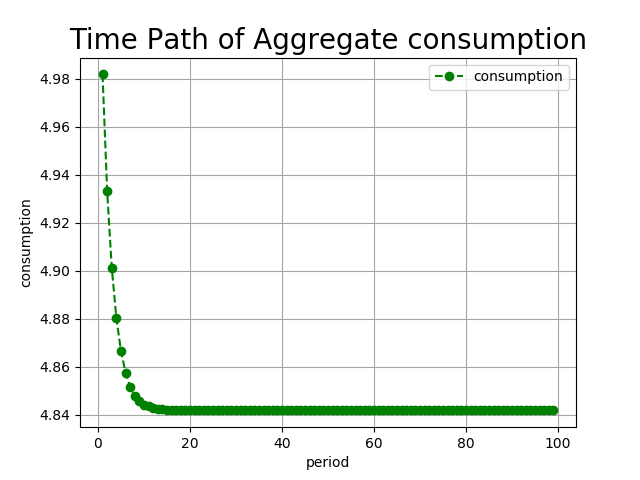
\includegraphics[scale=0.35]{tpi_C}
\\
\noindent\textbf{Problem 2(c)}\\
\begin{table}[htbp!]\centering
\begin{tabular}{|l|c|}\hline
 Savings Euler Error & $0.37$\\
 Labor Euler Error & $5.37e^{-8}$\\
 Last period saving & $0.24$\\
 Resource Constraint Error & $2.85e^{-7}$\\ \hline
\end{tabular}
\end{table}

\noindent\textbf{Problem 2(d)}\\
It takes 21 periods for the ec onomy to get within 0.0001 of the steady-state aggregate capital stock.
\end{document}
